%CONSIDERAÇÕES INICIAIS
% O ARQUIVO ORIGINAL NÃO É MEU, SÓ O RECHEIO (OBVIAMENTE, NÃO SOU OTÁRIO PRA PLAGIAR)
% SE VOCÊ QUER COPIAR, COPIE MESMO! WORD É PARA OS FRACOS, USE TEX E SEJA EFICIENTE, PORRA!
% É SÓ TROCAR O RECHEIO DAS COISAS, A ESTRUTURA DO TRABALHO É SUAVE DE ENTENDER E É BEM À PROVA DE NOOBS
% SE VOCÊ É NOOB: SINTO MUITO, SE FODEU. VOLTE AO M$ OFFICE QUE É O TEU LUGAR!
%
% RECOMENDO USAR ATOM OU SUBLIME TEXT COM O PLUGIN LATEX TOOLS E OS SNIPPETS QUE ESTÃO EM UM REPO DO GIT QUE
% EU AINDA VOU LINKAR AQUI
% VOCE TEM QUE TER O PACOTE MIKTEX BAIXADO E JA TER CONFIGURADO ELE PRA USAR ABNTEX2 E A PORRA TODA
% SENÃO NÃO VAI COMPILAR E VOCÊ VAI TER QUE VOLTAR PRO OFFICE E CONTAR PROS SEUS AMIGOS QUE VOCÊ
% FALHOU E É UMA DESONRA PARA OS PROGRAMADORES DO MUNDO INTEIRO. DESONRA PRA VOCÊ, DESONRA PRO SEU CÓDIGO!
%
% É ISSO AÍ, PARE DE PROCRASTINAR E FAÇA SEU TRABALHO. SEI QUE TÁ ATRASADO, RELAXA
% BOA SORTE!
\documentclass[
	% -- opções da classe memoir --
	12pt,				% tamanho da fonte
	openright,			% capítulos começam em pág ímpar (insere página vazia caso preciso)
	oneside,			% para impressão em verso e anverso. Oposto a oneside
	a4paper,			% tamanho do papel.
	% -- opções da classe abntex2 --
	%chapter=TITLE,		% títulos de capítulos convertidos em letras maiúsculas
	%section=TITLE,		% títulos de seções convertidos em letras maiúsculas
	%subsection=TITLE,	% títulos de subseções convertidos em letras maiúsculas
	%subsubsection=TITLE,% títulos de subsubseções convertidos em letras maiúsculas
	% -- opções do pacote babel --
	english,			% idioma adicional para hifenização
	french,				% idioma adicional para hifenização
	spanish,			% idioma adicional para hifenização
	brazil				% o último idioma é o principal do documento
	]{abntex2}

% ---
% Pacotes básicos
% ---
\usepackage{lmodern}			% Usa a fonte Latin Modern
\usepackage[T1]{fontenc}		    % Selecao de codigos de fonte.
\usepackage[utf8]{inputenc}		% Codificacao do documento (conversão automática dos acentos)
\usepackage{lastpage}			% Usado pela Ficha catalográfica
\usepackage{indentfirst}		    % Indenta o primeiro parágrafo de cada seção.
\usepackage{color}				% Controle das cores
\usepackage{graphicx}			% Inclusão de gráficos
\usepackage{microtype} 			% Para melhorias de justificação
\usepackage{afterpage}
\usepackage{amsmath}            % Pacote para fórmulas matemáticas
\usepackage{amssymb,url}
\usepackage{xcolor,tikz,bm,colortbl}
\usepackage[br]{nicealgo}       % Pacote para criação de algoritmos
\usepackage{customizacoes}
\usepackage[final]{pdfpages}
\usepackage{float}
\usepackage{xr}
\usepackage{nameref}
\usepackage{trivfloat}
\usepackage{listingsutf8}
% ---

% ---
% Pacotes adicionais, usados apenas no âmbito do Modelo Canônico do abnteX2
% ---
\usepackage{lipsum}				% Para geração de dummy text
% ---

% ---
% Pacotes de citações
% ---
\usepackage[brazilian,hyperpageref]{backref}	 % Paginas com as citações na bibl
\usepackage[alf]{abntex2cite}	% Citações padrão ABNT
% ---
% CONFIGURAÇÕES DE PACOTES
% ---
\trivfloat{quadro}
\floatstyle{plaintop} % Forçar posição da legenda para o topo
\restylefloat{quadro} % Forçar posição da legenda para o topo
\renewcommand{\listquadroname}{Lista de Quadros} % Forçar texto na Lista de Quadros
\renewcommand{\lstlistingname}{Algoritmo}
% ---
% Configurações do pacote backref
\renewcommand{\familydefault}{\sfdefault}
% Usado sem a opção hyperpageref de backref
\renewcommand{\backrefpagesname}{Citado na(s) página(s):~}
% Texto padrão antes do número das páginas
\renewcommand{\backref}{}
% Define os textos da citação
\renewcommand*{\backrefalt}[4]{
	\ifcase #1 %
		Nenhuma citação no texto.%
	\or
		Citado na página #2.%
	\else
		Citado #1 vezes nas páginas #2.%
	\fi}%
% ---

% ---
% Informações de dados para CAPA e FOLHA DE ROSTO
% ---
\titulo{TÉCNICAS ULTRALEVES PARA DETECÇÃO DE \textit{MALWARE} BASEADA EM
ASSINATURAS PARA REDES DE COMPUTADORES}
\autor{LUCAS THIAGO ASSUMPÇÃO GOUVÊA}
\local{Bauru}
\data{2016}
\orientador{Prof. Dr. Kelton Augusto Pontara da Costa}
\instituicao{%
  Universidade Estadual Paulista ``Júlio de Mesquita Filho''
  \par
  Faculdade de Ciências
  \par
  Ciência da Computação}
\tipotrabalho{Trabalho de Conclusão de Curso}
% O preambulo deve conter o tipo do trabalho, o objetivo,
% o nome da instituição e a área de concentração
\preambulo{Trabalho de Conclusão de Curso do Curso de Ciência da Computação da Universidade Estadual Paulista ``Júlio de Mesquita Filho'', Faculdade de Ciências, Campus Bauru.}
% ---


% ---
% Configurações de aparência do PDF final

% alterando o aspecto da cor azul
\definecolor{blue}{RGB}{41,5,195}

% informações do PDF
\makeatletter
\hypersetup{
     	%pagebackref=true,
		pdftitle={\@title},
		pdfauthor={\@author},
    	pdfsubject={\imprimirpreambulo},
	    pdfcreator={LaTeX with abnTeX2},
		pdfkeywords={abnt}{latex}{abntex}{abntex2}{trabalho acadêmico},
		colorlinks=true,       		% false: boxed links; true: colored links
    	linkcolor=blue,          	% color of internal links
    	citecolor=blue,        		% color of links to bibliography
    	filecolor=magenta,      		% color of file links
		urlcolor=blue,
		bookmarksdepth=4
}
\makeatother
% ---

% ---
% Espaçamentos entre linhas e parágrafos
% ---

% O tamanho do parágrafo é dado por:
\setlength{\parindent}{1.3cm}

% Controle do espaçamento entre um parágrafo e outro:
\setlength{\parskip}{0.2cm}  % tente também \onelineskip

% ---
% compila o indice
% ---
\makeindex
% ---

% ----
% Início do documento
% ----
\begin{document}

% Seleciona o idioma do documento (conforme pacotes do babel)
%\selectlanguage{english}
\selectlanguage{brazil}

% Retira espaço extra obsoleto entre as frases.
\frenchspacing

% ----------------------------------------------------------
% ELEMENTOS PRÉ-TEXTUAIS
% ----------------------------------------------------------
% \pretextual

% ---
% Capa
% ---
\imprimircapa
% ---

% ---
% Folha de rosto
% (o * indica que haverá a ficha bibliográfica)
% ---
\imprimirfolhaderosto*
% ---

% ---
% Inserir a ficha bibliografica
% ---

% Isto é um exemplo de Ficha Catalográfica, ou ``Dados internacionais de
% catalogação-na-publicação''. Você pode utilizar este modelo como referência.
% Porém, provavelmente a biblioteca da sua universidade lhe fornecerá um PDF
% com a ficha catalográfica definitiva após a defesa do trabalho. Quando estiver
% com o documento, salve-o como PDF no diretório do seu projeto e substitua todo
% o conteúdo de implementação deste arquivo pelo comando abaixo:
%
% \begin{fichacatalografica}
%     \includepdf{fig_ficha_catalografica.pdf}
% \end{fichacatalografica}

\begin{fichacatalografica}
	\sffamily
	\vspace*{\fill}					% Posição vertical
	\begin{center}					% Minipage Centralizado
	\fbox{\begin{minipage}[c][8cm]{15.5cm}		% Largura
	\small
	\imprimirautor
	%Sobrenome, Nome do autor

	\hspace{0.5cm} \imprimirtitulo  / \imprimirautor. --
	\imprimirlocal, \imprimirdata-

	\hspace{0.5cm} \pageref{LastPage} p. : il. (algumas color.) ; 30 cm.\\

	\hspace{0.5cm} \imprimirorientadorRotulo~\imprimirorientador\\

	\hspace{0.5cm}
	\parbox[t]{\textwidth}{\imprimirtipotrabalho~--~\imprimirinstituicao,
	\imprimirdata.}\\

	\hspace{0.5cm}
		1. Tags
		2. Para
		3. A
		4. Ficha
		5. Catalográfica
	\end{minipage}}
	\end{center}
\end{fichacatalografica}
% ---

% ---
% Inserir folha de aprovação
% ---

% Isto é um exemplo de Folha de aprovação, elemento obrigatório da NBR
% 14724/2011 (seção 4.2.1.3). Você pode utilizar este modelo até a aprovação
% do trabalho. Após isso, substitua todo o conteúdo deste arquivo por uma
% imagem da página assinada pela banca com o comando abaixo:
%
% \includepdf{folhadeaprovacao_final.pdf}
%
\begin{folhadeaprovacao}

  \begin{center}
    {\ABNTEXchapterfont\large\imprimirautor}

    \vspace*{\fill}\vspace*{\fill}
    \begin{center}
      \ABNTEXchapterfont\bfseries\Large\imprimirtitulo
    \end{center}
    \vspace*{\fill}

    \hspace{.45\textwidth}
    \begin{minipage}{.5\textwidth}
        \imprimirpreambulo
    \end{minipage}%
    \vspace*{\fill}
   \end{center}

   \center Banca Examinadora

   \assinatura{\textbf{\imprimirorientador} \\ Orientador}
   \assinatura{\textbf{Simone das Graças Domingues Prado} \\ Convidado 1}
   \assinatura{\textbf{João Paulo Papa} \\ Convidado 2}
   %\assinatura{\textbf{Professor} \\ Convidado 3}
   %\assinatura{\textbf{Professor} \\ Convidado 4}

   \begin{center}
    \vspace*{0.5cm}
    \par
    {Bauru, \_\_\_\_\_ de \_\_\_\_\_\_\_\_\_\_\_ de \_\_\_\_.}
    \vspace*{1cm}
  \end{center}

\end{folhadeaprovacao}
% ---

% ---
% Dedicatória
% ---
\begin{dedicatoria}
   \vspace*{\fill}
   \centering
   \noindent
   \textit{Dedico esse texto a todos que valorizam a liberdade e o conhecimento.}
   \vspace*{\fill}
\end{dedicatoria}
% ---

% ---
% Agradecimentos
% ---
\begin{agradecimentos}
Agradeço antes de tudo a meus pais, que me deram estrutura, amor, educação, força e qualidade de vida para que eu chegasse até aqui.
Agradeço por, num país tão desigual como o nosso, ter a chance e as condições de se formar numa universidade pública de qualidade. Tenho total consciência do quão privilegiado eu sou por ter tudo isso e por ter tudo o que tenho na vida.
Agradeço ao Kelton, meu orientador, por acreditar em mim e me auxiliar com sua paciência e o seu conhecimento no desenvolvimento deste trabalho
Agradeço também, à música, minha grande paixão, refúgio e meio de expressão, por ter sido crucial na manutenção da minha sanidade e da minha alegria nos momentos mais atormentados que cruzaram o meu caminho. Sem a música, a minha alma e creio que todo este mundo, estariam completamente desolados. Agradeço aos meus alunos por construírem arte e coisas positivas com o conhecimento que compartilhei com eles.
Agradeço à minha família pelo apoio e pelo carinho comigo durante toda a minha vida.
Agradeço aos amigos que tenho e que me estimam tanto. Em especial a Marcelo Montanha (meu irmão), Fernando Lima Fernandes, Michel Sunsin, Gabriel Naro, Caetano Ranieri, Luís Morais, Luís Paulo Jarussi, Felipe Leme e Victor Frascarelli por compartilharem os palcos comigo durante esses anos e à República Toca, por ter sido uma segunda casa e uma grande escola.
Agradeço à Barbara Toscano Barali, pelo amor e pela amizade, por todos os momentos compartilhados e pela ajuda e força inestimáveis que me deu nos meus dias mais tristes.
Agradeço a todos que sorriem ao se lembrar de mim e a todos que me fazem sorrir.
\end{agradecimentos}
% ---

% ---
% Epígrafe
% ---
\begin{epigrafe}
    \vspace*{\fill}
	\begin{flushright}
		\textit{Paciência, aplicação, perseverança e, acima de tudo, a vontade inabalável de atingir à meta. (Beethoven)}
	\end{flushright}
\end{epigrafe}
% ---

% ---
% RESUMOS
% ---

% resumo em português
\setlength{\absparsep}{18pt} % ajusta o espaçamento dos parágrafos do resumo
\begin{resumo}

Desde as origens da Internet, existe uma grande preocupação com a privacidade das comunicações e com a prevenção de danos causados por ataques que se aproveitam de vulnerabilidades nas redes corporativas e públicas. Com o aumento constante do uso de dispositivos conectados à internet e da intensidade e variedade de dados transmitidos entre as pessoas, o número de falhas de segurança em redes ainda é preocupante e tende a continuar subindo. Contudo, os pacotes de alguns programas utilizados nesses ataques, conhecidos como \textit{Malware}, possuem aspectos que são rastreáveis e que, quando incorporados aos métodos de busca dos sistemas de segurança, podem ajudar a detectar esses programas maliciosos antes que eles causem dano a outros pontos da rede infectados. A esses aspectos damos o nome de assinaturas de \textit{Malware} e o objeto de estudo deste trabalho são as técnicas de captura de \textit{Malware} que envolvem assinaturas, novas ferramentas do segmento e as tendências e que estão se apresentando no cenário tecnologico para esse tipo de abordagem. O trabalho propõe também a implementação de um ambiente de aplicação e testagem de assinaturas de \textit{Malware} sobre um conjunto de programas contendo traços de código malicioso, com o auxílio de ferramentas modernas que também são utilizadas por grandes empresas de segurança digital e desenvolvimento, além de um protótipo de textit{webservice} para testagem de assinaturas de \textit{malware} e verificação de arquivos \textit{online}.

\textbf{Palavras-chave:} Segurança de Redes, \textit{Malware}, Vírus de Computador.
\end{resumo}

% resumo em inglês
\begin{resumo}[Abstract]
\begin{otherlanguage*}{english}

Since the Internet's origins, there's a great preoccupation with the privacy of communications and with preventing damage caused by attacks that exploit vulnerabilities in corporative and private networks. With the increase in usage of internet connected devices and of the intensity and variety of transmitted data between people, the number of security flaws in networks is still worrisome and tends to keep growing. However, packages of some programs used in those attacks, known as malware, have traceable aspects that when incorporated to the search methods of security systems, might help detecting them before causing damage to other infected points ofthe network. To those aspects, we give the name of malware signatures, and the study object of this work are the malware capturing techniques involving signatures, new tools in the segment and the trends showing up in the technologic scenario to this kind of approach. The work also proposes the implementation of an environment to apply and test malware signatures on a set of programs containing traces of malicious code, with the help of modern tools that are also being used by big companies of digital security and development, and also a Web application prototype for online malware signature testing and file verification.

\textbf{Keywords:} Network security. Malware. Computer Viruses.

 \end{otherlanguage*}
\end{resumo}
% ---

% ---
% inserir lista de ilustrações
% ---
\pdfbookmark[0]{\listfigurename}{lof}
\listoffigures*
\cleardoublepage
% ---

% ---
% inserir lista de tabelas
% ---
\pdfbookmark[0]{\listtablename}{lot}
\listoftables*
\cleardoublepage
% ---

% ---
% inserir lista de quadros
% ---
\newpage % Forçar a lista de quadros em uma nova página
\phantomsection % Comando necessário caso o pacote hyperref seja utilizado, visando a corrigir o link
\addcontentsline{toc}{chapter}{\listquadroname} % Adicionar no Sumário um capítulo cujo nome está contido na variável listquadroname
\listofquadros % Adiciona lista de quadros
\cleardoublepage

% ---
% inserir lista de abreviaturas e siglas
% ---
% ---

% ---
% inserir o sumario
% ---

\pdfbookmark[0]{\contentsname}{toc}
\tableofcontents*
\cleardoublepage
% ---

% ----------------------------------------------------------
% ELEMENTOS TEXTUAIS
% ----------------------------------------------------------
\pagestyle{simple}

% ----------------------------------------------------------
% Introdução (exemplo de capítulo sem numeração, mas presente no Sumário)
% ----------------------------------------------------------

\chapter{INTRODUÇÃO}
\label{c.introducao}

A presença das redes de computadores no cotidiano vem aumentando de modo muito
veloz há anos e apresentou um crescimento em especial com o advento das redes
sem fio e da produção massiva e a queda do custo de dispositivos portáteis
capazes de se conectarem à internet. De maneira proporcional, aumentaram-se
também os riscos relacionados à segurança de redes e à privacidade de
informações de diversas espécies que trafegam por entre elas e seus usuários.
Numa proposição inicial, este trabalho define como \textit{Malware} todo tipo de
programa que seja capaz de alterar o comportamento de um software num
dispositivo conectado a uma rede qualquer, feito com o desejo de vender
informações de usuários, causar desordem, roubar credenciais, enviar \textit{spams},
alimentar motores de otimização de busca (SEO) com informações falsas sobre
visitas a páginas da Web ou ainda de chantagear usuários, como foi o caso do
\textit{malware} japonês denominado \textit{Kenzero}, que publicava históricos de navegação
juntamente com a identificação de seus usuários, a menos que os mesmos
pagassem 1500 ienes para que seus dados fossem retirados do acesso ao público.
SAWLE et al. (\citeyear{sawle14}).

De acordo com IDIKA (\citeyear{idika07}), pode-se classificar os tipos de
métodos de detecção de maneira mais rudimentar em duas categorias: detecção
baseada em anomalia e detecção baseada em assinatura. A detecção por anomalia
é uma técnica que consiste em treinar um algoritmo de detecção para que ele
“saiba” o que constitui o comportamento normal de um programa, para que ele
possa decidir sobre a periculosidade dos programas a serem inspecionados. Essa
mesma abordagem também dá origem a uma técnica muito similar conhecida como
detecção baseada em especificações, onde levantam-se especificações e
conjuntos de regras para que a partir daí defina-se o comportamento de um
programa normal. A técnica de detecção por assinaturas, por sua vez, envolve a
caracterização do que já seria sabidamente malicioso para encontrar traços
semelhantes e encontrar os programas anômalos. Todas as técnicas citadas acima
podem ser aplicadas com um de três modos diferentes, sendo eles análise
estática, análise dinâmica e análise híbrida, onde a análise estática num
contexto de detecção por assinaturas, verificaria aspectos estruturais de
programas inspecionados, como sequências de \textit{bytes}, e a análise dinâmica
buscaria informações de maneira concorrente ao tempo de execução do programa.
Em suma, a análise estática procura investigar o programa antes que ele seja
executado, e a análise dinâmica atua ou na execução do programa, ou depois que
ele já foi executado. As técnicas híbridas são simplesmente combinações dessas
duas anteriores, juntando informações estáticas e dinâmicas para que se
conclua um parecer sobre a maliciosidade dos códigos analisados.

Dessa maneira, é possível exemplificar as técnicas de detecção com a figura 1:

\begin{figure}[H]
\caption{\small Classificação das técnicas de detecção de \textit{Malware}}
\centering
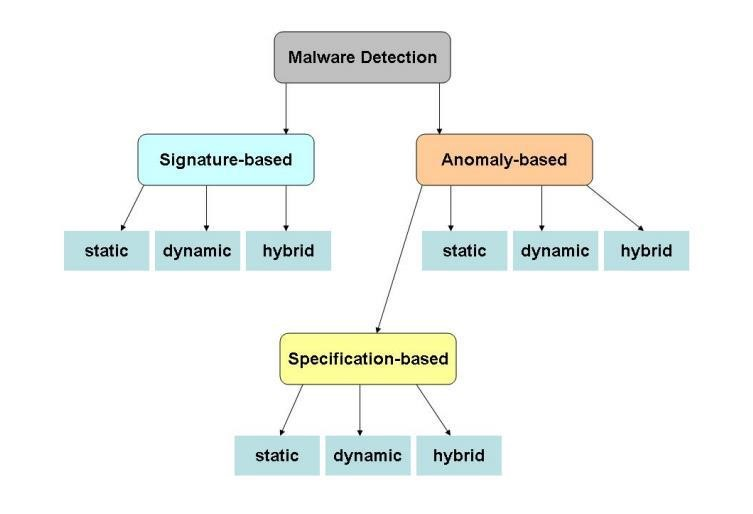
\includegraphics[scale=0.8]{figs/fig1}
\label{f.metodos_deteccao_01}
\legend{\small Fonte: Elaborada pelo autor.}
\end{figure}

Nesta seção do texto, ainda será explicado o problema que o projeto se propõe a resolver, os objetivos esperados para a implementação e a justificativa para o estudo que se desenvolveru no tema. No capítulo 2
encontra-se todo o referencial teórico que permeia os conceitos de redes, segurança de redes, famílias de
\textit{malware} e outros conceitos relacionados ao projeto. No capítulo 3 estão as informações sobre as ferramentas que foram utilizadas na fase de implementação, documentada no capítulo 4. O capítulo 5 conclui o texto com algumas considerações sobre estudos futuros e os resultados obtidos em vários aspectos do projeto.

\section{Problema}
\label{c.problema}

Os dispositivos móveis atuais ainda não possuem capacidade computacional disponível para que se façam varreduras constantes que utilizem as técnicas de
detecção dinâmicas em seus respectivos sistemas à procura de código malicioso,
e com a abrangência da internet se tornando cada vez mais expressiva, o dano
em potencial que um \textit{malware} pode causar a um determinado indivíduo, ou ainda
em grupos massivos também torna-se mais preocupante. Sob a ótica de Szewczyk
(\citeyear{szewczyk12}), as redes de computadores, principalmente sem fio, começam a apresentar
problemas de vulnerabilidade a partir do momento da compra do \textit{hardware}
necessário para implementação da rede e da configuração desse equipamento,
onde muitas vezes os vendedores destes produtos tentam passar a ideia de que
os equipamentos por si são capazes de blindar uma rede contra qualquer
intrusão, a fim de obter sucesso comercial valendo-se da ingenuidade de
usuários leigos no assunto de segurança de redes. As técnicas de detecção por
assinatura, apesar de não serem as mais eficazes à disposição, são muito mais
simples de se implementar e resolverem o problema da infecção por \textit{malwares}
conhecidos ou ainda \textit{malwares} novos com características semelhantes às dos
conhecidos.

\section{Objetivos e justificativa}
\label{s.objetivos}

\subsection{Objetivo Geral}
\label{s.objetivog}

Analisar o resultado da ação de diferentes técnicas de detecção de \textit{malware}
baseadas em assinatura num ambiente de testes para obter métricas relevantes
quanto à eficiência nas varreduras realizadas, número de falsos positivos
encontrados e se possível determinar qual delas é a mais apropriada para uso
em ambientes \textit{mobile} e de redes de computadores em geral.
 
\subsection{Objetivos Específicos}
\label{s.ojetivosp}

- Para embasar o projeto, foi levantado um histórico sobre segurança em redes
  de computadores e assuntos correlacionados principalmente às técnicas de
  detecção a serem estudadas.

- Montar um ambiente para que ele seja populado com conjuntos de programas a
  serem investigados e executar diferentes algoritmos para que posteriormente
  classifiquem-se seus resultados. Por questões de relevância, o escopo do
  trabalho envolverá sistemas \textit{Windows} e \textit{Android} pois a maioria dos usuários
  comuns utiliza estes sistemas operacionais.

- Comparar todos os métodos previamente escolhidos e testados para apresentar
  suas respectivas características e desempenhos.


\subsection{Justificativa}
\label{s.justificativa}

O desenvolvimento de novas técnicas de segurança computacional, bem como a
análise e aprimoramento de técnicas já construídas anteriormente, representam
sempre um avanço na área de segurança de redes, pois todo tipo de sistema
operacional possui alguma deficiência no quesito de segurança, haja visto que
mesmo agências de inteligência como a NSA enfrentam de tempos em tempos
problemas envolvendo vazamentos de dados e intrusões. De acordo com HASSAN (\citeyear{hassan10}), os tipos de ataque mais poderosos e bem
sucedidos ocorrem de dentro da rede, pois em diversas situações, o
administrador de rede confia em todos os usuários internos e não suspeita de
ataques vindos de seu próprio lado. Por isso, é sempre um investimento
desenvolver e manter uma política de aprimorar as defesas das redes de
computadores. O contexto do projeto é o da esfera do usuário comum, que
utiliza dispositivos comuns mas também é alvo de ataques que às vezes são
menores e até inofensivos, que contudo, ocorrem com frequência.
\chapter{OBJETIVOS}
\label{c.objetivos}

 

\subsection{Objetivo Geral}
\label{s.objetivog}

Analisar o resultado da ação de diferentes técnicas de detecção de \textit{malware}
baseadas em assinatura num ambiente de testes para obter métricas relevantes
quanto à eficiência nas varreduras realizadas, número de falsos positivos
encontrados e se possível determinar qual delas é a mais apropriada para uso
em ambientes mobile e de redes de computadores em geral.
 
\subsection{Objetivos Específicos}
\label{s.ojetivosp}

- Para embasar o projeto, será levantado um histórico sobre segurança em redes
  de computadores e assuntos correlacionados principalmente às técnicas de
  detecção a serem estudadas.

- Montar um ambiente para que ele seja populado com conjuntos de programas a
  serem investigados e executar diferentes algoritmos para que posteriormente
  classifiquem-se seus resultados. Por questões de relevância, o escopo do
  trabalho envolverá sistemas \textit{Windows} e \textit{Android} pois a maioria dos usuários
  comuns utiliza estes sistemas operacionais.

- Comparar todos os métodos previamente escolhidos e testados para apresentar
  suas respectivas características e desempenhos.


\subsection{Justificativa}
\label{s.justificativa}

O desenvolvimento de novas técnicas de segurança computacional, bem como a
análise e aprimoramento de técnicas já construídas anteriormente, representam
sempre um avanço na área de segurança de redes, pois todo tipo de sistema
operacional possui alguma deficiência no quesito de segurança, haja visto que
mesmo agências de inteligência como a NSA enfrentam de tempos em tempos
problemas envolvendo vazamentos de dados e intrusões. De acordo com Hassan e
Muhammad (\citeyear{hassan10}), os tipos de ataque mais poderosos e bem
sucedidos ocorrem de dentro da rede, pois em diversas situações, o
administrador de rede confia em todos os usuários internos e não suspeita de
ataques vindos de seu próprio lado. Por isso, é sempre um investimento
desenvolver e manter uma política de aprimorar as defesas das redes de
computadores. O contexto do projeto é o da esfera do usuário comum, que
utiliza dispositivos comuns mas também é alvo de ataques que às vezes são
menores e até inofensivos, que contudo, ocorrem com frequência.



\chapter{FUNDAMENTAÇÃO TEÓRICA}
\label{c.fundamentacao}

Neste capítulo é apresentado o plano de fundo teórico que envolve os tópicos
pertinentes ao trabalho, destacando as definições e conceitos essenciais dos
seguintes assuntos: Redes de Computadores, Internet, Segurança em redes de
Computadores (estado da arte), \textit{Malware} e suas respectivas técnicas de
detecção.
\section{Redes de Computadores e Internet}
\label{s.teoria_redes_internet}

Segundo o trabalho de KUROSE (\citeyear{kurose09}), pode-se definir a Internet
como a rede de computadores que interconecta milhões de dispositivos
computacionais ao redor do mundo. Há pouco tempo a gama de dispositivos
conectados à internet era mais baixa e se resumia a servidores e computadores
de mesa. Hoje pode-se ver que cada vez mais dispositivos não tradicionais
estão sendo ligados à internet. Assim, defini-se como sistemas finais, ou
hospedeiros, quaisquer dispositivos que possuam tal capacidade de conexão. Em
julho de 2008 estimavam-se 600 milhões de sistemas finais ligados à internet
sem contar dispositivos que são conectados de maneira intermitente (como
laptops e smartphones). Quando sistemas finais se comunicam, trocam arquivos
segmentados, que denominam-se como pacotes, por meio de enlaces de comunicação
(links), que podem ser físicos ou por ondas, no caso de redes sem fio e via
rádio. Os dispositivos periféricos que são responsáveis por essa comunicação
são chamados comutadores de pacotes, vistos comumente como roteadores e
switchs. O que torna essa comunicação válida entre tantos dispositivos
diversos são os protocolos de rede, como TCP/IP. Tais protocolos apenas
definem a estrutura dos pacotes que serão trocados e a classificação dos dados
dentro destas estruturas. Dessa maneira, os comutadores de pacotes conseguem
interagir sem problemas e dividir as cargas da rede com eficiência. Neste
trabalho não se faz necessária uma abordagem mais profunda sobre estruturas de
pacotes e de componentes mais específicos da rede, haja visto que o foco do
trabalho é voltado para segurança em redes e uma revisão completa sobre
fundamentos básicos de redes não elucida conteúdos dessa vertente. Os pacotes
ainda serão citados no decorrer do trabalho e terão seus conceitos devidamente
esclarecidos na seção apropriada. A ideia geral de redes de computadores
suficiente para esse trabalho pode ser ilustrada com a seguinte imagem:

\begin{figure}[H]
\caption{\small Alguns componentes da internet}
\centering
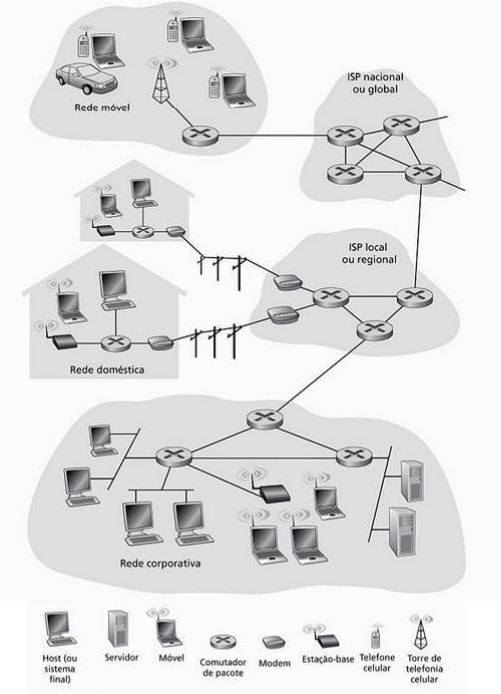
\includegraphics[scale=1.3]{figs/fig3.JPG}
\label{f.internet_01}
\legend{\small Fonte: Kurose (2009)}
\end{figure}

\section{Segurança em redes de computadores}
\label{s.seguranca}

Ainda no material de Kurose pode-se definir vários conceitos em segurança de
redes. A ideia em si vem de imaginar que as pessoas desejam se falar através
da internet, por exemplo, e que essas pessoas não queiram que ninguém mais
seja capaz de interceptar esses dados mesmo que elas estejam conectadas em
locais considerados inseguros, que deixam computadores serem publicamente
utilizados. Além disso, imaginar que as pessoas também querem garantir que as
mensagens trocadas não sejam originadas de um intruso, ou passem por um
intruso na rede. Com essa ideia pode-se elencar as propriedades necessárias
para uma comunicação considerada \emph{segura}. São elas:

\begin{itemize}
\item[-] Confidencialidade: A garantia de que somente respectivos remetentes e destinatários sejam capazes de ver e entender o conteúdo das mensagens transmitidas.
\item[-] Autenticação do ponto final: Remetentes e destinatários precisam ter meios de confirmar a identidade uns dos outros durante uma comunicação.
\item[-] Integridade da mensagem: Além de identificarem uns aos outros, os envolvidos na comunicação querem assegurar que o conteúdo que enviem seja exatamente o conteúdo que as outras partes recebam. As mensagens podem se corromper durante uma comunicação tanto por acidentes, como por má intenção de intrusos na rede.
\item[-] Segurança Operacional: Qualquer empresa atualmente vai ter uma rede local conectada à rede pública. Os mecanismos responsáveis por filtrar o que a rede local vai receber da rede pública são chamados mecanismos de segurança operacional, como firewalls, que são servidores que se posicionam entre as duas redes e intermedeiam a comunicação entre elas, e também como sistemas de detecção de intrusão, foco maior do trabalho, que são sistemas que analisam os pacotes de maneira mais profunda e os identificam para separar e tratar pacotes potencialmente suspeitos.
\end{itemize}

Qualquer ação de um intruso na rede configura uma falha na presença de um ou
mais dos quesitos elencados acima; quando ocorre tal brecha e um usuário
estranho consegue acesso não autorizado a uma rede, ele ganha muitas
possibilidades de uso pra essa rede. Um invasor pode agir de modo passivo
apenas monitorando as comunicações que pode ver, ou então agir com um caráter
mais nocivo e alterar os conteúdos que acessa, seja corrompendo, alterando ou
removendo arquivos, senhas e dados diversos. Os sistemas de detecção de
intrusão buscam maneiras de identificar acessos ilegais e tráfego de dados
estranhos na rede. \subsection{Estado atual da área de segurança de redes}
\label{sub:estado_da_arte}

De acordo com Hurd (\citeyear{hurd15}) uma área bastante promissora é a de
\emph{Cyber Higiene}, e seus aspectos incluem gerenciamento e proteção de credenciais,
auditoria de roubo de credenciais e dados analíticos sobre comportamento de
acesso do usuário, sendo esta última subárea a que demonstra a maior parcela
de progresso recente e num futuro de médio prazo. Nesse segmento, o conceito
de usuário pode ser especificado além do usuário comum, classificando novos
perfis como atacantes e autores (programadores). O comportamento envolve
características como duração do tempo de acesso, preferência de dispositivo
utilizado, utilização de navegador e outras diversas informações sobre as
atividades desenvolvidas por um usuário e quais seriam seus fins. Utilizando a
internet como ``observatório'' , a análise do comportamento de
usuários tem sofrido uma revolução em virtude do crescimento da internet das
coisas, onde cada vez mais objetos estão conectados à rede, com grande parte
destes objetos sempre reportando informações, como sensores e câmeras de
trânsito.


\section{Malware}
\label{s.malware_01}

O conceito de \textit{Malware} já foi abordado de maneira mais rudimentar na introdução
do trabalho. Porém, como o viés do projeto caminha muito próximo de
classificações mais profundas desse tópico, faz-se necessário recorrer a uma bibliografia mais
completa sobre os processos relacionados ao \textit{Malware}. Na pesquisa desenvolvida
por SAHEED(\citeyear{saeed13}), pode-se aproveitar muitas informações sobre o
patamar do desenvolvimento deste tipo de \textit{software}. De acordo com pesquisas
levantadas pela McAfee, esses programas continuam a se tornar mais numerosos
dia-a-dia, sendo encontrados novos ``indivíduos'' aos milhares. Em
contrapartida, pesquisadores e laboratórios especializados em segurança
aprimoram novos métodos para construir \textit{anti-malware} mais eficiente e mais
autônomo. A seguir, diferenciam-se os tipos de \textit{Malware} com base nas técnicas de
criação dos mesmos, separando-os por técnicas de ofuscamento, métodos de
invocação, plataforma de atividade, abrangência e técnicas de propagação. Nem
todo \textit{software} malicioso é executado de dentro de máquinas infectadas;
atualmente a maioria dos ataques são originários da internet, pois as
vulnerabilidades encontradas são mais proeminentes do que em ambientes de rede
local, em virtude de a internet ser um espaço, de modo geral, público,
beneficiando atacantes que tenham meios de acessar um sistema alvo
remotamente. Um sistema de detecção de \textit{malware} tem majoritariamente duas
tarefas: busca e análise, ou seja, saber encontrar material não confiável e
saber identificar com precisão que o material em questão realmente possui
traços nocivos de código, ou faz com que algum outro programa apresente
comportamento considerado anormal.

\subsection{Técnicas de criação}
\label{ss.tecnicas}

Para criar esse tipo de código, atacantes utilizam de vários meios desde a
inserção de pequenos pedaços de código em outros programas, até a algoritmos
de alta complexidade, feitos com o intuito de esconder o \textit{malware} ou torná-lo
\emph{polimórfico}. Um \textit{malware} que se classifique como polimórfico consiste em
um programa capaz de trocar pedaços do código sem mudar a semântica e o
resultado da execução a cada infecção, para driblar verificações de sintaxe,
geralmente com a ajuda de técnicas avançadas de encriptação. \textit{Malwares}
polimórficos são o grande ponto fraco das técnicas de detecção por assinatura,
pois eles tornam inviável a geração de assinaturas únicas para classificação
do código malicioso. Pode-se dizer que um \textit{Malware} é \emph{ofuscado} quando ele é
polimórfico ou \emph{metamórfico}, onde o código original é transformado em
algo funcionalmente equivalente, porém muito mais difícil de se compreender
quando lido. As técnicas utilizadas para que isso ocorra são a utilização de
código morto, que é uma grande parcela de código que não faz absolutamente
nada, acoplado ao código malicioso para mascará-lo, ou também a transportação
de código, que consiste em realizar um grande número de ``jumps'' no programa,
porém sem alteração no fluxo de controle do mesmo.

\subsection{Malware baseado em rede}
\label{ss.malware_rede}

Para dar início à classificação dos tipos de \textit{Malware}, primeiro observa-se com
destaque aqueles que se utilizam da rede como meio de propagação e de atuação.
Nesse segmento, é possível identificar o que são os \textit{Adwares}, \textit{Spywares}, \textit{Cookies},
\textit{Backdoors}, \textit{Trojans}, \textit{Sniffers}, \textit{Spam} e \textit{Botnet}.

\textit{Spyware} é um tipo de \textit{malware} que se instala de maneira secreta num computador,
com o objetivo de coletar informações sobre o uso de determinados programas ou
sites visitados por um indivíduo sem o conhecimento do mesmo. Curiosamente,
até mesmo grandes empresas como Google e Microsoft se utilizam desse tipo de
\textit{Malware} para coletar informações de seus clientes.

\textit{Adwares} são feitos com a finalidade de servirem como atalhos publicitários
para outros programas que têm seu desenvolvimento mantido com fundos oriundos
de propaganda na internet. Por natureza, não são essencialmente danosos a
sistemas e no máximo causam transtorno às pessoas por apresentarem anúncios
indesejados, entretanto, existem algumas variações nessa família de \textit{malware}
que possuem \textit{spyware} acoplados juntamente com as propagandas, invadindo a
privacidade dos usuários.

\textit{Cookies}, na verdade, são informações de usuário guardadas pelos navegadores de
internet; eles servem primeiramente como meio de autenticação e armazenamento
de configurações entre cliente e servidor. Um cookie é um pequeno arquivo de
texto com essas informações, e na maioria das vezes vai ter um prazo de
validade fixado pelo servidor que o usuário acessa. Também não são danosos,
mas os \textit{cookies} são usados por \textit{spywares} e também no roubo de credenciais de
usuários.

\textit{Backdoors} ou \textit{Trapdoors} são código malicioso atrelado a aplicações ou sistemas
operacionais que concedem a alguém acesso a um sistema sem que seja necessário
passar por métodos comuns de autenticação. Eventualmente esses programas
também podem ser usados como meio para conseguir acesso remoto a sistemas.

Um \textit{Trojan Horse} (cavalo de tróia), ou apenas \textit{Trojan}, descreve um programa que
aparenta ser útil ou inofensivo, mas que ao ser executado pode corromper dados
ou roubar informações. Um \textit{Trojan} é desenvolvido para que o usuário, além de
não suspeitar dele, seja levado a executá-lo por curiosidade, então é muito
comum ver esse tipo de programa escondido em arquivos multimídia que vão
seduzir algum nicho de usuários.

\textit{Sniffers} são capazes de monitorar e armezenar dados a respeito do tráfego de
uma rede. Eles capturam os pacotes que estão sendo trocados e os decodificam
para ganhar acesso aos dados crus dos campos dos pacotes. \textit{Sniffers} podem ser
usados como um passo inicial para uma invasão, para que posteriormente sejam
obtidas senhas e outras informações confidenciais que sejam alvo de um
atacante.

O \textit{Spam} talvez seja o tipo de \textit{malware} mais conhecido por usuários mais leigos;
basicamente é um pacote de \textit{software} com a funcionalidade de transmitir
mensagens em larga escala via \textit{e-mail}. O impacto negativo do \textit{spam} é a
possibilidade de lentidão causada pelo alto número de requisições que será
realizado por ele para os servidores, atrapalhando o recebimento de mensagens
mais relevantes e poluindo as caixas de \textit{e-mail}. Embora seja uma prática muito
mal vista na internet, nos Estados Unidos o \textit{spam} é legalizado, graças ao ato
CAN-SPAM, desde 2003.

\textit{Botnet} não é na verdade um \textit{malware} de código, mas uma coleção de computadores
infectados e que são controlados remotamente por um atacante que pode usá-los
para realizar atos maldosos sem que seja preciso se autenticar nessas
máquinas. Esse é o conceito por trás dos ataques de negação de serviço (DoS),
onde um grande número de máquinas controladas sobrecarrega um determinado
serviço na rede com um número absurdo de requisições aos servidores.(SAHEED, 2013)

\subsection{Malware Comum}
\label{ss.malware_comum}

O \textit{Malware} comum, em contraste com o de rede, é feito para ser executado em
ambiente local sem a necessidade de qualquer conexão a rede, pois também pode
ser propagado via dispositivos físicos como pendrives, HDs externos e
periféricos com \textit{software} malicioso embarcado. Nessa categoria, classificam-se os vírus, \textit{worms} e bombas lógicas.

Vírus de computador é um conceito que muitas vezes acaba generalizando o
\textit{Malware}. É muito comum um usuário que foi infectado apenas com \textit{adware} dizer
que ``está com vírus no PC'' e assim segue; Na verdade, um vírus de computador
é um código capaz de se replicar durante a infecção em qualquer programa ou
documento. Por exemplo, sistemas Windows em muitas mídias se utilizam de um
arquivo ``autorun.inf'' para automatizar a execução de tarefas para montagem
de pastas ou imagens de disco. Logo, um código maldoso que possa se acoplar
silenciosamente a esse tipo de arquivo, com certeza conseguirá infectar um
sistema Windows.

Os Worms são códigos capazes de se replicar em múltiplas máquinas de modo
independente, isto é, sem precisar se atrelarem a um determinado programa para
iniciar seu ciclo de vida. Eles podem, entre outras coisas, consumir a banda
da rede e privar o usuário infectado de utilizá-la, além de criarem várias
cópias de si para aumentar a taxa de programação. Esta última característica é
o que os \textit{softwares} de anti-vírus utilizam para identificar Worms; se um
arquivo está se repetindo muitas vezes com atributos iguais, ele é considerado
suspeito nesses sistemas de detecção.

A bomba lógica é um \textit{software} que permanece quieto até que se atinja uma
determinada condição. Para isso, o programa fica apenas checando a data do
sistema até que seja a data especificada e só então ele vai, de fato, executar
seu código.(SAHEED, 2013)

Dadas essas classificações, pode-se ilustrar os tipos de \textit{malware} e suas características com o seguinte quadro:

\begin{quadro}[h]
\caption{\small Famílias de \textit{Malware} e fatores comparativos}
\centering
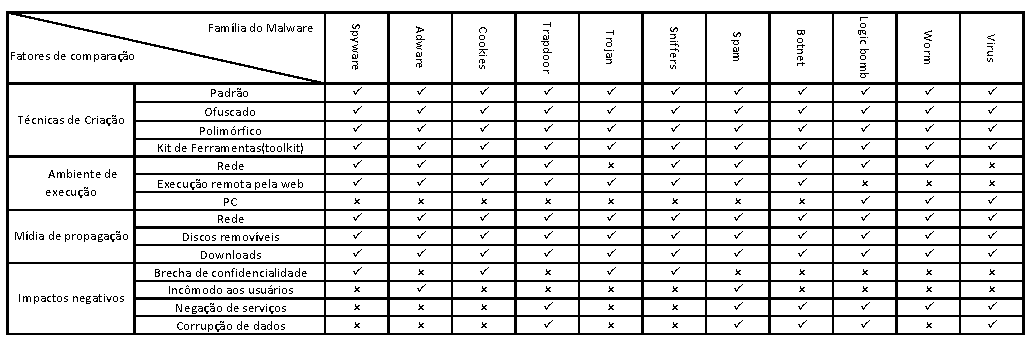
\includegraphics{figs/tabela.pdf}
\label{f.tabelamalware}
\legend{\small Fonte: Saeed (2013) (traduzida pelo autor).}
\end{quadro}
\subsection{Exemplos de Código de Malware} % (fold)
\label{ssub:exemplos_malware}

Alguns \textit{malwares} acabam tendo seu código aberto e disponibilizado para estudos, ora por vontade de seus próprios autores, ou por vazamento de informações feito por outros \textit{Hackers} interessados em tornar público esse tipo de informação. Nesta seção encontram-se algumas explicações sobre a arquitetura interna dos \textit{malwares} e trechos de código-fonte obtidos a partir de pesquisas em repositórios públicos da \textit{web} 

- Citar os repositórios
- Imagens do código dos malwares


% subsubsection subsubsection_name (end)

\section{Detecção}
\label{s.deteccao}

Nesta seção, é exposto o estado atual das tecnologias de
detecção e para onde elas estão caminhando no futuro. O trabalho de
Baddar et al. (\citeyear{baddarxx}) nos mostra uma perspectiva bastante atual do cenário e
de como funcionam, de modo geral, os processos de detecção das anomalias. Um
sistema de detecção pode agir em ambiente de rede, verificando as
características do tráfego da rede, ou em nível de aplicação, onde vai varrer
os dados do disco a procura de assinaturas conhecidas de anomalia ou de
comportamentos fora do normal. A detecção por comportamento anômalo precisa
ser capaz de filtrar casos anômalos isolados, denominados como anomalias
pontuais, de casos com suspeita mais palpável de anomalia, que pode-se chamar de
anomalia de contexto. Uma anomalia pontual pode ser exemplificada do seguinte
modo: uma tentativa de acesso de um usuário num sistema corporativo não é, a
princípio, um ato que possa ser classificado como anômalo; porém, se essa
mesma tentativa se repete várias vezes em horários não condizentes com o
expediente comercial, pode haver alguém suspeito tentando roubar as
credenciais desse usuário. As figuras abaixo exemplificam as ideias de
anomalia pontual e contextual:

\begin{figure}[H]
\caption{\small Exemplo de anomalia pontual}
\centering
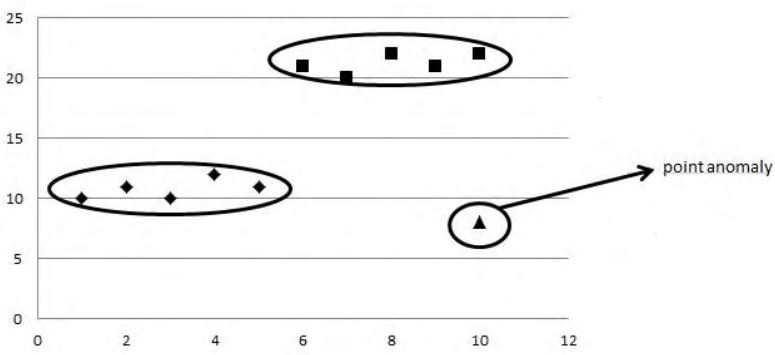
\includegraphics[scale=0.5]{figs/anomalia_pontual.JPG}
\label{f.anomalia_pontual}
\legend{\small Fonte: Baddar. (\citeyear{baddarxx})}
\end{figure}

\begin{figure}[H]
\caption{\small Exemplo de anomalia contextual}
\centering
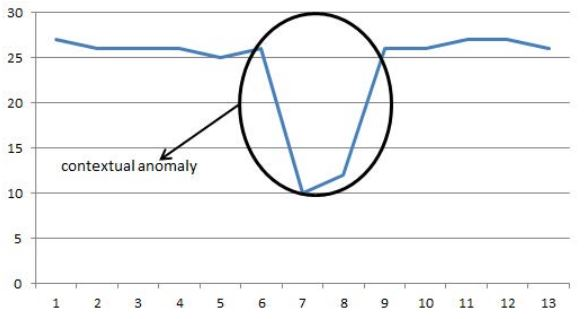
\includegraphics[scale=0.5]{figs/anomalia_contextual.JPG}
\label{f.contextual}
\legend{\small Fonte: Baddar. (\citeyear{baddarxx})}
\end{figure}

\subsection{Detecção baseada em funcionalidade}
\label{ss.deteccao_funcionalidade} Destaca-se esse segmento em especial pois é
daqui que se origina a ideia de detecção baseada em assinaturas e em
comportamentos. A detecção baseada em assinaturas compara casos suspeitos com
uma relação já conhecida de código comprovadamente nocivo, que fica armazenada
geralmente num banco de dados da empresa que desenvolve o sistema de detecção.
Motores de busca de anti-vírus são o exemplo mais clássico de detecção baseada
em assinaturas. Numa outra abordagem, a detecção por comportamento vai tentar
``aprender'' como vive um programa normal dentro do sistema, e como é o ciclo
de um programa suspeito, geralmente recorrendo a dados de tempo de execução
dos programas que estão sendo processados e classificando essas
características com o auxílio de técnicas como aprendizado de máquina e redes
neurais (BADDAR, \citeyear{baddarxx}). A maior parte do conjunto recente das aplicações de detecção
em nível de rede tem adotado a abordagem do aprendizado de máquinas para
detectar \textit{software} por comportamento, quando em nível de rede. Em nível de
aplicação, a grande maioria também procura traçar perfis de comportamento
utilizando técnicas de detecção em modo dinâmico como pode-se ver nos quadros
abaixo:

\begin{quadro}[h]
\caption{\small Tecnologias recentes de detecção em nível de rede}
\centering
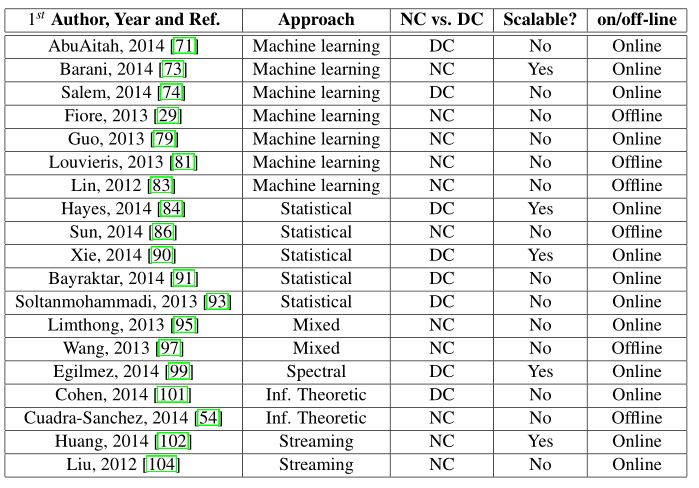
\includegraphics[scale=0.7]{figs/tabela_deteccao_nivel_rede.JPG}
\label{f.tabeladeteccao_rede}
\legend{\small Fonte: Baddar. (\citeyear{baddarxx})}
\end{quadro}

\begin{quadro}[h]
\caption{\small Tecnologias recentes de detecção em nível de aplicação}
\centering
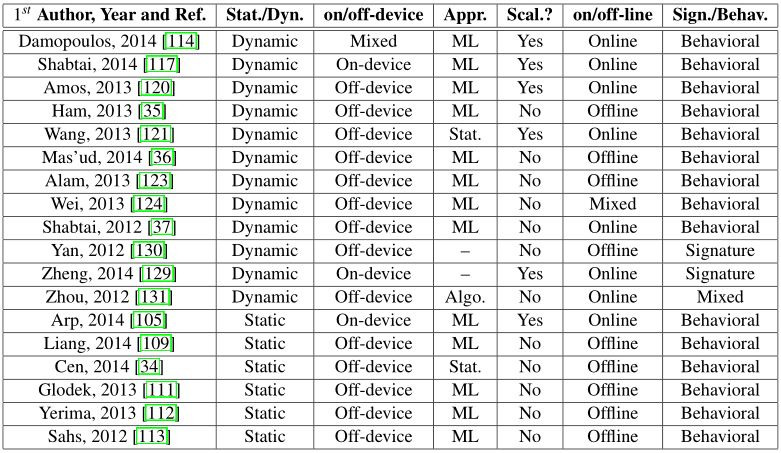
\includegraphics[scale=0.7]{figs/tabela_deteccao_nivel_aplicacao.JPG}
\label{f.tabeladeteccao_app}
\legend{\small Fonte: Baddar. (\citeyear{baddarxx})}
\end{quadro}









\externaldocument{desenvolvimento}
\chapter{METODOLOGIA}
\label{c.metodologia}

O estudo foi segmentado de acordo com as seguintes etapas:

\begin{itemize}
	\item[-] Levantamento bibliográfico
	\item[-] Análise e desenvolvimento das técnicas de detecção baseadas em assinatura utilizadas atualmente
	\item[-] Implementação Computacional
	\item[-] Análise dos resultados e conclusão da monografia.
\end{itemize}
A confecção da monografia ocorreu juntamente com o andamento das demais
etapas definidas durante toda a extensão do projeto. A ideia foi utilizar
máquinas virtuais e emuladores para implementar em caráter de teste os
algoritmos de detecção baseados em assinatura sobre um conjunto de programas
contendo alguns programas já infectados com amostras de \textit{malware} diversas para
observar, em termos gerais, a eficiência do tempo de execução dos algoritmos e
suas respectivas taxas de sucesso. Como o ambiente pode ser montado em qualquer
máquina que suporte a plataforma Windows e emulador Android, então não há
necessidade de que se reserve material da UNESP para uso exclusivo do projeto.
A figura 5 ilustra o planejamento do projeto:
\begin{figure}[H]
\caption{\small Estrutura do projeto}
\centering
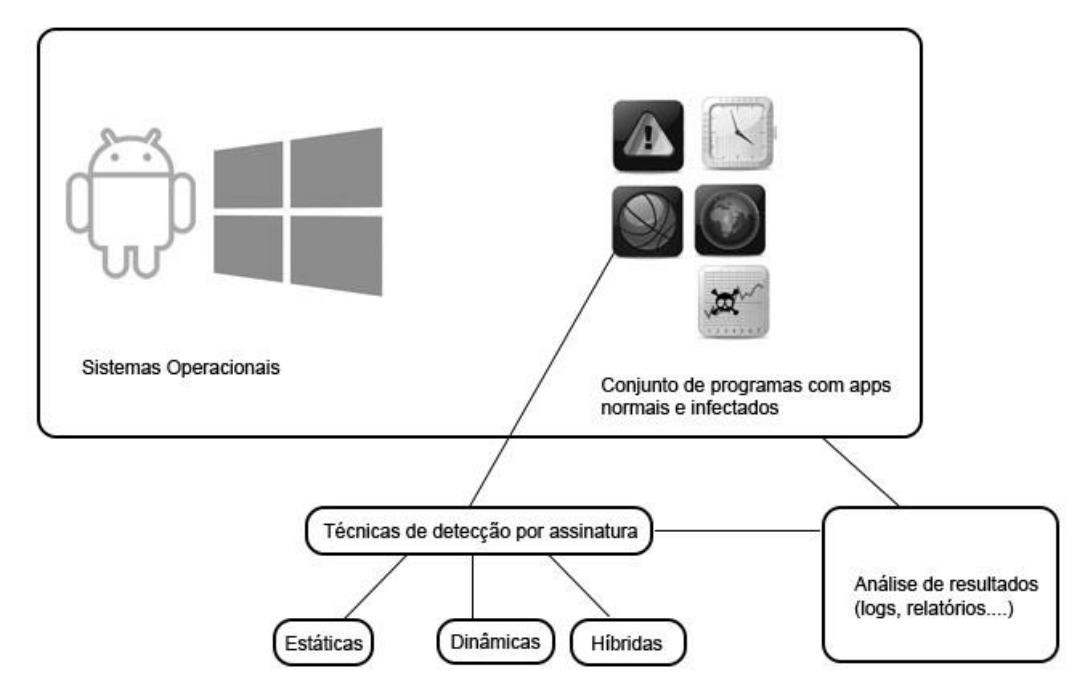
\includegraphics[scale=0.4]{figs/fig2}
\label{f.estrutura_projeto}
\legend{\small Fonte: Elaborada pelo autor.}
\end{figure}

O fluxo de desenvolvimento do projeto consiste na aplicação de um índice de
regras de detecção do Yara, construído a partir da conversão de arquivos
contendo bases de assinaturas do Clam AV para arquivos contendo regras de
detecção do Yara, sobre o conjunto de amostras vivas de \textit{malware} obtidas
nos repositórios citados na seção do desenvolvimento do projeto. As varreduras
são feitas via linha de comando e para agilizá-las, além do uso de índices para
agrupar regras, também pode-se automatizar as varreduras em grupos maiores de
arquivos aplicando um pouco de \textit{shell script}. Os resultados das
varreduras serão armazenados em arquivos de texto que irão conter todos os
atributos analisados a cada arquivo a respeito de uma determinada regra. Vamos
explicar com um pouco mais de detalhe como ficam caracterizadas as infecções nos
\textit{logs} de resultados, com casos de teste envolvendo expectativas de
resultados positivos, falso-positivos e negativos. Ao final da seção de
desenvolvimento, também foi explicada a ideia da aplicação \textit{web} para
varreduras remotas e manipulação de regras do Yara.

\section{Materiais Utilizados}
\label{l.material}

\subsection{Servidor Local} % (fold)
\label{sub:servidor}

Foi utilizada uma máquina com 4GB de RAM, 1TB de armazenamento e sistema operacional Windows 10 de arquitetura 64 bits.

\subsection{Yara}
\label{sub:Yara}

Yara é uma ferramenta de código aberto recentemente desenvolvida, cujo intuito é
auxiliar desenvolvedores a identificar e classificar amostras de
\textit{malware}. Ele é construído em C, porém, com o auxílio de algumas
bibliotecas, há a possibilidade de incorporá-lo em scripts de outras linguagens,
como Python. Segundo ALVAREZ (\citeyear{yararules}), o funcionamento do Yara consiste em comparar
regras criadas pelo desenvolvedor que descrevem famílias de \textit{malware},
com o código de executáveis quaisquer, ou também de arquivos comprimidos em
alguns formatos comuns. As regras podem variar bastante em nível de complexidade
e mapearem diversas características do comportamento dos executáveis, que serão
detalhadas posteriormente. O projeto no momento encontra-se bastante popular e o
programa está sendo utilizado como ferramenta de construção de assinatura de
\textit{malware} por desenvolvedores de diversos grupos importantes no ramo,
entre eles:
\begin{itemize}
	\item[-] ActiveCanopy
	\item[-] Adlice
	\item[-] CrowdStrike FMS
	\item[-] Fox-IT
	\item[-] Heroku
	\item[-] Kaspersky Lab
	\item[-] Picus Security
	\item[-] ReversingLabs
	\item[-] Symantec
	\item[-] ThreatStream, Inc.
	\item[-] Trend Micro
	\item[-] VirusTotal Intelligence
	\item[-] We Watch Your Website
\end{itemize}

O Yara foi utilizado no presente trabalho de conclusão de curso como meio de
aplicação dos algoritmos de assinatura nos programas que serão examinados. Com
o auxílio de \textit{scripts} desenvolvidos em Python, será simulada uma varredura nesse
conjunto de programas aplicando regras obtidas através de sites como o
\href{yararules.org}{Yara Rules} e o
\href{http://sanesecurity.com/usage/signatures/}{Sane Security}, que
disponibilizam sem custo algum assinaturas de milhões de códigos maliciosos já
capturados pela web. Com esse grande arsenal de assinaturas de \textit{malware}, é
possível testar com certa completude as técnicas e assinaturas que são
desenvolvidas no mercado e utilizadas nos sistemas de detecção de intrusão.

\subsubsection{Regras de detecção do Yara}
\label{l.regrasdyara}
O Yara funciona interpretando arquivos que contém características que possivelmente
apontam para o padrão dos elementos da família do \textit{malware} que deve ser
isolado. As regras são escritas com uma sintaxe simples que remete à
construção de uma estrutura de dados em C, contendo strings a serem comparadas
tanto em formato texto quanto hexadecimal, conjuntos de strings, endereços da
memória que ficarão sob monitoramento, limitações de tamanho de arquivo,
expressões regulares, pontos de entrada de execução e variáveis externas.
Todos esses dados do arquivo examinado podem ativar condições, listadas na
construção dessas regras, que vão determinar se o arquivo corresponde ou não à
família definida nas regras de detecção. Para exemplificar mais claramente a
construção e o funcionamento das regras, seguem alguns exemplos de código
obtido do repositório do projeto \href{yararules.com}{Yara Rules} (yararules.com) no
\href{github.com}{Github}, ilustrados nas figuras 6 e 7.

\begin{figure}[H]
	\centering
	\caption{Regra de detecção para o \textit{malware} ``Zeus''.}
	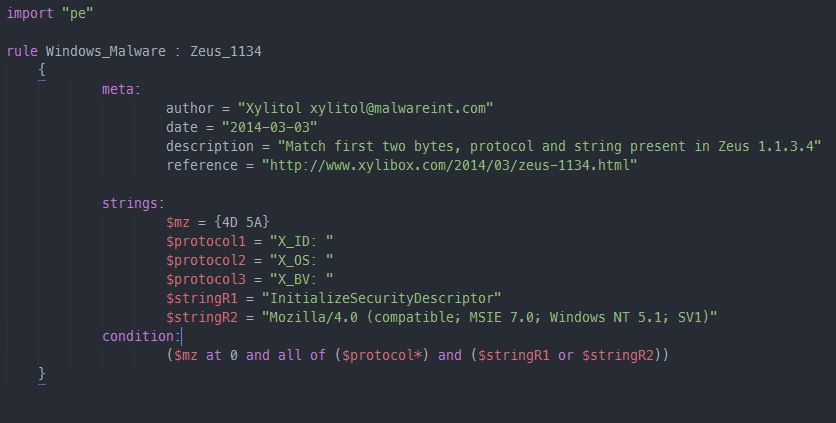
\includegraphics[width=0.95\textwidth]{figs/zeus}
	\label{f.regrazeus}
	\legend{Fonte: elaborada pelo autor}
\end{figure}

Na imagem acima ilustra-se um exemplo de uma descrição para o \textit{malware} chamado
``Zeus'' (também conhecido como ``RPG'', ``ZBot'', ``Infostealer'', entre
outros), que é membro da família dos \textit{Trojans}. Segundo informações da
\href{www.wiki-security.com}{Wiki Security} \footnote{www.wiki-security.com} (\citeyear{wikisecurity}) os danos
causados por ele incluem roubo de informações pessoais como senhas de email e de
bancos, para posteriormente efetuarem-se transferências para ``contas-mula'' que
lavariam o dinheiro das vítimas até que ele chegasse aos atacantes. O
\textit{malware} foi escrito majoritariamente em C com alguns pequenos trechos
em php, e seu código fonte, vazado em 2011, pode ser encontrado neste outro
repositório público do Github (https://github.com/Visgean/Zeus). Como
pode-se observar, a regra escrita para marcar o trojan verifica os dois
primeiros \textit{bytes}, \textit{strings} e o protocolo utilizados por uma
determinada versão do ``Zeus'' e fica ativa quando a primeira e uma das outras
duas condições são satisfeitas.

Outro exemplo de regra de detecção envolvendo parâmetros semelhantes aos
anteriores é a que descreve o \textit{malware} ``Lenovo
Superfish'' (LENOVO, \citeyear{lenovosuperfish}) ; na verdade esse é o nome de um serviço
que vinha embutido em algumas séries de equipamentos lançados pela fabricante
Lenovo entre 2014 e 2015, cuja meta era ajudar consumidores a encontrar produtos
similares aos que eles buscavam pela web. Esse serviço possuía uma
vulnerabilidade de protocolos que foi explorada na criação do \textit{malware}
homônimo. No caso, as características que estão sendo mapeadas são novamente os
dois primeiros \textit{bytes} do programa, porém com strings em formato e
encodificações diferentes das encontradas na regra anterior, como segue na figura 7:

\begin{figure}[H]
	\centering
	\caption{Regra de detecção do ``Superfish''}
	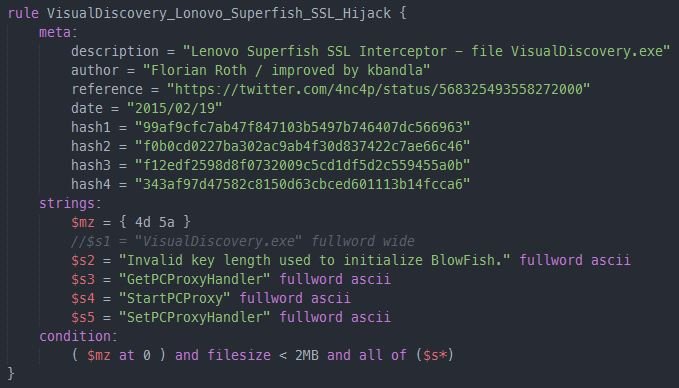
\includegraphics[width=0.95\textwidth]{figs/superfish}
	\label{f.superfish}
	\legend{Fonte: elaborada pelo autor}
\end{figure}

As regras que serão aplicadas no decorrer do projeto serão unificadas num arquivo
de índice, compiladas com o uso de um \textit{script} em Python para a
interpretação do Yara e combinadas com o conjunto completo de arquivos de uma só
vez, pois o próprio Yara já possui métodos implementados que possibilitam
varreduras de maneira recursiva.

\subsection{\textit{Logs} de resultados do Yara} % (fold)
\label{sub:logs_de_resultados_do_yara}

As varreduras efetuadas pelo Yara podem ter seus resultados gravados em arquivos
de texto para análise posterior, que podem também denominarem-se
\textit{logs}, que por sua vez retornam um  breve dicionário de strings com formato exemplificado no Algoritmo 1:
\renewcommand{\thelstlisting}{\arabic{lstlisting}}
\begin{lstlisting}[caption=Conteúdo dos arquivos de resultado de varredura, label=resultyara]
{
'tags': ['mal', 'ware'],
'matches': True,
'namespace': 'default',
'rule': 'regras_compiladas',
'meta': {},
'strings': [(81L, '$a', 'abc'), (141L, '$b', 'def')]
}
\end{lstlisting}

Respectivamente, segue o que cada parâmetro representa:
\begin{itemize}
	\item '\textit{tags}': conjunto dos nomes dos programas maliciosos que estão sendo buscados

	\item '\textit{matches}': True significa positivo para infecção
	
	\item '\textit{namespace}': Nome do conjunto ao qual a regra escrita pertence (padrão: \textit{default})

	\item '\textit{rule}': Arquivo com as regras compiladas para aplicação

	\item '\textit{meta}': metadados do arquivo

	\item '\textit{strings}': conjunto de strings para comparação dentro do objeto de varredura
\end{itemize}

Existe também a possibilidade de utilizar-se outros módulos para verificação e
isolamento de outros atributos do arquivo como, por exemplo, detecção do uso de
compressão de executáveis, que é uma técnica comum empregada no desenvolvimento
de \textit{malware}. Por questões de viabilidade e complexidade do projeto,
procurou-se aplicar uma abordagem mais simples, sem a realização de testes de
implementação dos referidos módulos.

\subsection{Python}
\label{sub:python}

É uma linguagem de programação cujo desenvolvimento ocorre desde 1989. No ano de
1994, foi lançada a primeira distribuição da versão 1.0 oficial da linguagem e
sua versão mais recente foi lançada em setembro de 2015. Para as necessidades do
presente projeto, foi adotada a versão 2.7 da linguagem, por suportar a
implementação dos \textit{scripts} do Yara e também ser a distribuição mais
estável da linguagem, segundo o \textit{site} oficial da linguagem.\footnote{www.python.org} O
Yara suporta integração com scripts feitos tanto em código C puro como em
Python, porém a escolha da linguagem se deu principalmente pela quantidade de
material disponível, onde a grande maioria de scripts já prontos e documentados
foi feita em Python,  e pelo fácil acesso à comunidade de desenvolvimento caso
fosse necessário. As implementações em C são mais comuns em âmbito corporativo,
onde se constroem módulos mais otimizados para uso em varreduras de
\textit{malware} numa escala mais elevada e o desempenho e a confidencialidade
do código tornam-se um fator mais significativo na aplicação das regras.

\subsection{Clam AV}
\label{sub:clamav}

O Clam AV é um antivírus de código aberto que possui um sistema muito
interessante para a montagem de sua base de dados de assinaturas. O
\textit{Community Threat Tracking System} funciona coletando os dados de
infecções ocorridas nos sistemas dos usuários e aprimorando suas assinaturas
automaticamente com base nos dados estatísticos que a comunidade fornece. As
bases buscam evidenciar quais \textit{malwares} estão mais ativos no momento, e
tornam todas as suas descobertas públicas. Os usuários têm a opção de enviarem
dados tanto anonimamente, quanto com um identificador único para cada
instalação, e tais dados não são comercializados com terceiros, ou monetizados
de alguma outra forma, todas as análises feitas por eles são apenas um serviço
gratuito prestado à comunidade \textit{open source}. No projeto que foi
desenvolvido, utilizaram-se bases de dados com assinaturas utilizadas pelo Clam
AV em suas próprias varreduras em \textit{scripts} que as reconhecem,
descomprimem e convertem para regras do Yara, que a partir de então podem ser
editadas ou testadas isoladamente a critério do desenvolvedor.

\chapter{DESENVOLVIMENTO}
\label{c.Desenvolvimento}

- Montagem do ambiente de testes com o Yara [ x ]

- Obtenção de regras de detecção [ x ]

- Testes iniciais [ x ]

- Testagem completa e análise de resultados [ ]

\chapter{Cronograma}
\label{c.cronograma}

O cronograma proposto para o caminhar do trabalho fica definido dentro das seguintes etapas:
\begin{itemize}
	\item[-] Etapa 1: Revisão Bibliográfica
	\item[-] Etapa 2: Análise e desenvolvimento das técnicas que serão estudadas
	\item[-] Etapa 3: Implementação computacional
	\item[-] Etapa 4: Análise de resultados e desenvolvimento da monografia
\end{itemize}

\begin{figure}[h]
\centering
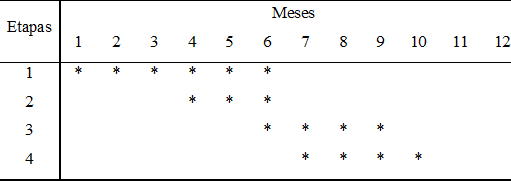
\includegraphics[scale=0.7]{figs/cronograma.png}
\label{f.cronograma}
\end{figure}






\chapter{CONCLUSÃO}
\label{c.conclusao}

A questão do aprimoramento das técnicas de segurança de redes e de informação
permanecerá relevante por muito tempo, em virtude do fato de que estamos
inseridos em um mundo que cada vez mais produz e depende de tecnologia e também
apresenta este mesmo comportamento quanto ao volume e à variedade de dados que
trafegam pela \textit{internet}. Com os estudos levantados e uma análise do
cenário atual da computação, pode-se afirmar que as técnicas estudadas e
aplicadas no desenvolvimento deste projeto estão, em termos de desempenho,
chegando ao seu máximo, pois a manipulação de assinaturas de \textit{malware}
implica características no processo de detecção que limitam uma possível
abordagem com o uso de técnicas de programação mais inovadoras. Embora a
eficácia das ferramentas atualmente empregadas seja satisfatória e as mesmas
apresentem uma boa precisão de detecção, estamos sempre atuando num contexto do
que pode-se chamar de `pós-infecção' ou pelo menos de uma infecção iminente,
onde os arquivos maliciosos já estão trafegando por pontos de rede ou até mesmo se encontram
latentes dentro dos ambientes vulneráveis infiltrados, seja por estarem à espera de um
comando do usuário ou por terem execução agendada. O panorama dos estudos nesse
segmento da área de segurança de redes está, em maior parte, tomando um viés
para a prevenção de infecções e episódios de vulnerabilidade, onde os métodos de
detecção de intrusão por anomalia e comportamento apresentam a vantagem de
estarem constantemente procurando se antecipar a possíveis ataques e a novas
formas de quebra de segurança, com a utilização de conceitos como redes neurais,
grafos, e até mesmo aprendizado de máquina.

No âmbito mais prático do desenvolvimento do projeto, observou-se que a abertura
para a criação e melhoria de técnicas envolvendo assinaturas é relativamente
recente, e as ferramentas encontradas e utilizadas para tais fins não são
voltadas para o público mais leigo e, talvez, curiosos e entusiastas do assunto,
haja visto que mesmo uma ferramenta como o Yara, cujo intuito é tornar essa
manipulação de assinaturas mais simplificada, requer uma configuração que exige
um razoável conhecimento de utilização de terminais e linhas de comando, e
afinidade com alguma linguagem de programação de alto ou médio nível para a
construção dos scripts de varredura ou conversão de bases de assinaturas. Foi
pensando nesse aspceto que se desenvolveu a ideia da aplicação \textit{online}
com um sistema capaz de automatizar as tarefas de manuseio de assinaturas de
\textit{malware}, para que as pessoas possam, além de testar a confiabilidade de
arquivos encontrados na \textit{internet}, ter um ponto de partida para conhecer
essa área da computação e também tentar colocar um pouco desse conhecimento em
prática de uma maneira colaborativa. O código-fonte do protótipo da aplicação
encontra-se hospedado \href{https://github.com/ltgouvea/TCC }{neste
repositório},  aberto para quaisquer desenvolvedores que queiram dar andamento
ao projeto caso se interessem. Já há serviços de varredura de \textit{malware}
gratuita disponíveis pela \textit{internet}, então o interesse maior no
desenvolvimento dessa aplicação é o diferencial que existiria na manipulação de
assinaturas de modo colaborativo, possivelmente anônimo e montando bases de
dados automaticamente no módulo de conversão de regras descrito no capítulo de
desenvolvimento do projeto. O resultado final foi uma aplicação funcional das
técnicas propostas no projeto que pode ser utilizada isoladamente, sem o auxílio
de outros \textit{softwares} antí-virus quaisquer, e posteriormente ampliada ou
incorporada no segmento de uma aplicação \textit{online} similar à ideia descrita
durante o desenvolvimento do projeto.


% ---
% Capitulo com exemplos de comandos inseridos de arquivo externo
% ---
% ---

% ----------------------------------------------------------
% ELEMENTOS PÓS-TEXTUAIS
% ----------------------------------------------------------
\postextual
% ----------------------------------------------------------

% ----------------------------------------------------------
% Referências bibliográficas
% ----------------------------------------------------------
\pagestyle{empty}
\bibliography{references} % o arquivo de bibliografia deve ser importando nessa linha sem o .bib

% ----------------------------------------------------------
% Glossário
% ----------------------------------------------------------
%
% Consulte o manual da classe abntex2 para orientações sobre o glossário.
%
%\glossary

%---------------------------------------------------------------------
% INDICE REMISSIVO
%---------------------------------------------------------------------
\phantompart
\printindex
%---------------------------------------------------------------------

\end{document}
